% Security evaluation, experiment 15.
%
% Figures: sec-grid.pdf is the 2x2 used by the paper; the four standalone
% sec-{vp,dmp,compsimp,spec}.pdf are the same panels if separate floats are
% wanted instead. Produced by
%   gem5-DIT/benchmarks/expedite_security/plot_paper_figs.py
% from paper_experiments/15-security-evaluation/data/results.csv, and land in
% that experiment's figures/ as sec-vp, sec-dmp, sec-compsimp, sec-spec.
% sec-grid-col.pdf is the same 2x2 laid out for a single-column float.
%
% Every number below is from that CSV. Compiler cbec54a0866f, gem5-DIT
% 25675e4aff03 plus the probes, Neoverse-V2 FDP, SE mode.

\subsection{Security Evaluation}\label{sec:eval:soundness}

We construct one microbenchmark per gated optimization and run each on three
designs: a \emph{baseline} with the mode switches removed, \emph{Apple-style
DIT} (\texttt{-{}-apple}), the gem5 model of Apple's design, whose
\texttt{msr dit} is unordered and establishes the mode only when it commits,
and ExpeDITe, whose switch is renamed and whose clear
is deferred until it cannot be squashed. Each microbenchmark must leak on the
baseline, leak under \texttt{-{}-apple}, and not leak under ExpeDITe.

The baseline is the same binary with the two \texttt{msr dit} instructions
omitted, so its column is the optimization running unobstructed. It cannot be
obtained by leaving the switch flag off: with no flag the simulator selects a
serialising drain, and the region is still live.

We observe microarchitectural state directly in the simulator rather than
through a timing channel. That makes the leak counts upper bounds on what an
attacker recovers, and correspondingly makes ExpeDITe's zeros stronger than a
timing measurement would be, since they count events an attacker would first
have to detect.

\begin{figure*}[t]
  \centering
  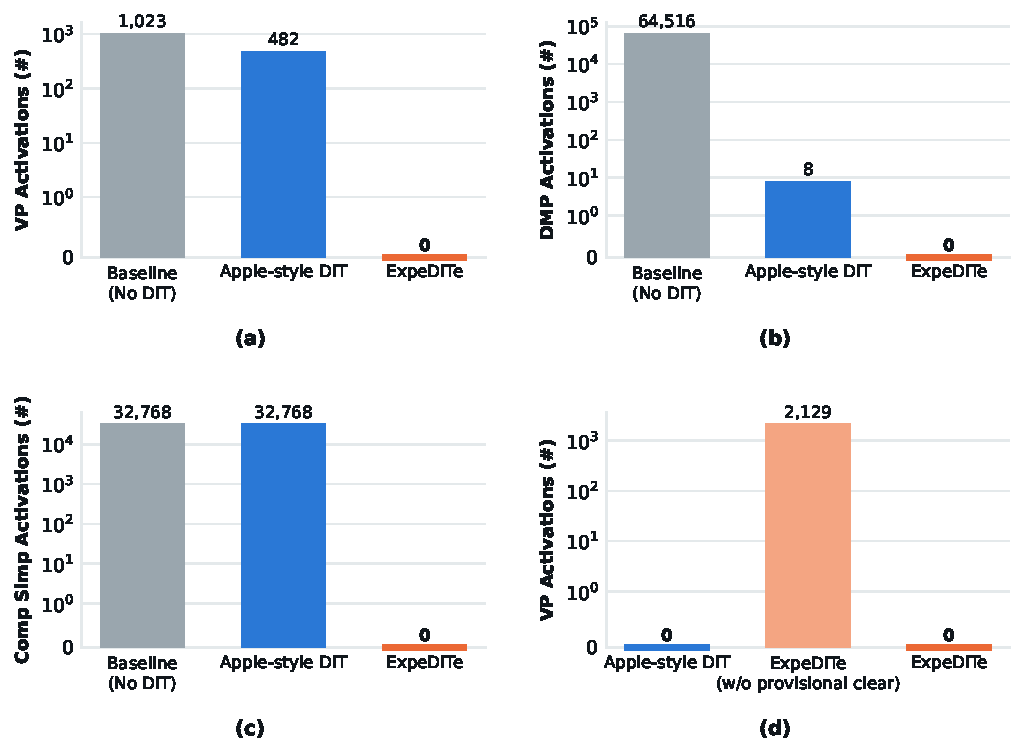
\includegraphics[width=\textwidth]{figures/sec-grid.pdf}
  \caption{Each gated optimization acting inside the DIT region. (a)~activations
  of the value predictor on the secret loads, net of the training loads the
  probe predicts outside any region; (b)~DMP activations, each one a prefetch
  of a line addressed by a secret pointer; (c)~computation simplifications,
  that is multiplies that ran with operand-dependent latency, of the 32{,}768
  in the region. In (a)--(c) the baseline is the same binary
  with the mode switches removed, and \emph{Apple-style DIT} is the gem5 model
  of Apple's design (\texttt{-{}-apple}): the switch is unordered against older
  instructions and establishes the mode only when it commits. Every
  optimization activates on the baseline and under Apple-style DIT, and none
  activates under ExpeDITe. (d)~value-predictor activations on loads that were
  architecturally \emph{inside} the DIT region and executed only
  speculatively, behind a clear that never architecturally executed: loads that
  should have been gated. Apple-style DIT reads zero here for a structural
  reason rather than as a defence, and \S\ref{sec:eval:spec} says why.}
  \label{fig:sec-grid}
\end{figure*}

\subsubsection{Load value prediction}\label{sec:eval:vp}

Listing~\ref{lst:sec-vp} is the gadget. Sixteen loads of one hot line from
sixteen distinct PCs sit directly behind the mode switch, dispatched alongside
it. The value is identical on every pass, which is the stride-0 case the
predictor reaches confidence on fastest, so if the predictor is permitted to act
it will and the prediction count is a direct readout of whether it was
permitted.

Under \texttt{-{}-apple} the switch is not ordered against older instructions,
so loads dispatched with it issue before it executes and read the mode it is
about to replace. Figure~\ref{fig:sec-grid}(a) shows 482 predicted secret loads,
against 1{,}023 with no protection at all and \textbf{zero} under ExpeDITe. A
region-scoped counter that needs no baseline subtraction corroborates it:
\texttt{predictionsInDitSequence} reads 485 under \texttt{-{}-apple} and 0 under
ExpeDITe.

\begin{lstlisting}[float=t, caption={The value-prediction microbenchmark. Sixteen
stride-0 loads of one hot line, from sixteen distinct PCs, dispatched alongside
the mode switch so some issue before it executes.}, label=lst:sec-vp]
for (int r = 0; r < ROUNDS; r++) {
  guard = *cold;         // cold miss: keeps
                         // the window open
  set_dit();             // msr DIT, #1

  /* the shadow: 16 loads, 16 PCs, one
     line, same value every round */
  v0 = *hot;  v1 = *hot;
  v2 = *hot;  v3 = *hot;
  /* ... v4 .. v15 ... */

  clear_dit();           // msr DIT, #0
}
\end{lstlisting}

\subsubsection{Data memory-dependent prefetching}\label{sec:eval:dmp}

Listing~\ref{lst:sec-dmp} plants Augury's activation pattern: an array of
pointers walked in order and \emph{never dereferenced by the program}. The DMP
dereferences them anyway, scanning every line it fills for pointer-shaped words
and prefetching what they address, so the set of resident lines after the walk
is a function of the secret pointer values. Targets are shuffled across a
\SI{1}{\mebi\byte} arena so a prefetch of a pointed-to line cannot be mistaken
for next-line prefetching, and the array is sized past the L2 so its lines are
genuinely filled; the DMP only scans on a fill.

This gate differs from the other two. Value prediction and computation
simplification key on the instruction's \texttt{DitCC} operand, because they
must match the Arm DIT instruction list; the prefetch clause of
E1.2.5 is written over the DIT \emph{sequence}, so this gate keys on region
membership and is stamped on the request in the load-store queue.
Figure~\ref{fig:sec-grid}(b): the unprotected walk issues 64{,}516 prefetches of
secret-addressed lines. Apple-style DIT issues 8, from the one fill in
8{,}192 whose request was stamped before the mode took effect. ExpeDITe drops
every one of its 8{,}191 fills at the gate and issues none.

\begin{lstlisting}[float=t, caption={The DMP microbenchmark. An array of secret
pointers is summed, never followed; every fetch of a pointed-to line is the
prefetcher's doing.}, label=lst:sec-dmp]
void victim(const uint64_t *const *aop,
            int entries)
{
  uint64_t acc = 0;

  /* sums the POINTERS; nothing here
     follows one */
  for (int i = 0; i < entries; i++)
    acc += (uint64_t)(uintptr_t)aop[i];

  sink += acc;
}
\end{lstlisting}

\subsubsection{Computation simplification}\label{sec:eval:compsimp}

Listing~\ref{lst:sec-compsimp} places eight independent multiplies by a register
holding zero immediately behind the mode switch. The simplifier shortcuts a
multiply whose operand is 0 or 1 and retires it early, so the multiply's
\emph{latency becomes a function of its operand}, which is the channel THOR
attacks on Intel AMX. Figure~\ref{fig:sec-grid}(c): all 32{,}768 multiplies in
the region run with operand-dependent latency under \texttt{-{}-apple}, exactly
as they do unprotected, and none do under ExpeDITe.

Two measurement notes belong with that figure. First, the counter counts issue
attempts rather than instructions: \texttt{trySimplify} runs once per issue, and
\texttt{-{}-apple} squashes the payload whenever its switch commits, so each
multiply is simplified five to six times and the factor moves with the gadget.
We therefore report how many multiplies \emph{ran} with operand-dependent
latency, which cannot exceed how many exist. Second, this leak has a cause
beyond the window: the simplifier is the only consumer of the DIT gate that
skips the readiness test, so it acts on a stale mode where every other consumer
fails safe.

\begin{lstlisting}[float=t, caption={The computation-simplification
microbenchmark. Eight independent multiplies by a register holding zero, issued
in the switch's shadow; \texttt{z} is opaque to the compiler.},
label=lst:sec-compsimp]
for (int i = 0; i < ITERS; i++) {
  guard = *cold;         // cold miss
  set_dit();             // msr DIT, #1

  /* 8 independent multiplies by zero */
  p0 = a * z;  p1 = a * z;
  p2 = a * z;  p3 = a * z;
  p4 = a * z;  p5 = a * z;
  p6 = a * z;  p7 = a * z;

  clear_dit();           // msr DIT, #0
}
\end{lstlisting}

\subsubsection{Speculation}\label{sec:eval:spec}

The three leaks above are all on the speculation path. Each happens while the
mode switch is still in flight, and the work is flushed when the switch commits;
architecturally nothing leaked, and every committed multiply in
\S\ref{sec:eval:compsimp} ran gated. That is precisely what E1.2.5 forbids, as
it counts instructions that only ever execute speculatively as part of the DIT
sequence: a design that establishes the mode at commit has already leaked by the
time it fixes anything.

Listing~\ref{lst:sec-spec} asks the converse question. A clear that never
architecturally executes must not un-gate what follows it. The victim has a
secret-dependent early exit, so the compiler-placed \texttt{msr dit, \#0} on
that path runs whenever the branch mispredicts, and everything behind it is
architecturally still inside the sequence.

Figure~\ref{fig:sec-grid}(d) counts exactly the loads that matter: those
architecturally inside the region that executed only speculatively, behind a
clear that never architecturally executed. Under ExpeDITe the clear's register
holds a conservative 1 from rename until the clear provably cannot be squashed,
and \textbf{none} of the 475 activations issued in a clear's shadow is
in-sequence. Publish that same clear as soon as it executes -- the identical
binary, one design decision removed -- and 2{,}129 are. That is what the
provisional clear buys.

Apple-style DIT reads zero, and the reason is worth stating because it is not a
defence. It establishes the mode only when the write commits, so a clear on a
wrong path never takes effect and the case simply does not arise for it. The
same property that makes it safe here is what makes it leak in
\S\ref{sec:eval:vp}--\ref{sec:eval:compsimp}: a \emph{set} that has not
committed has not taken effect either, and the in-region work behind it runs
unprotected. A design that resolves the mode at commit does not solve the
speculation problem; it moves it from the exit of a region to the entrance.

\begin{lstlisting}[float=t, caption={The speculation microbenchmark. The early
exit is guarded by a secret bit, so the clear the compiler places on that path
executes whenever the branch mispredicts.}, label=lst:sec-spec]
void victim(const uint64_t *secret,
            int n, int start)
{
  uint64_t acc = 0;

  for (int i = 0; i < n; i++) {
    uint64_t v = secret[(start + i) & MASK];
    acc += v ^ 0x5a5a5a5a;
    if (v & 1) {         // secret-dependent
      sink ^= acc;       // volatile: keeps
      return;            // this a branch
    }                    // -> msr DIT, #0
    acc ^= v * 3;        //    on this path
  }
  sink ^= acc;
}
\end{lstlisting}
